\documentclass[conference]{IEEEtran}

\makeatletter
% IEEEtran.cls defines \labelindent for backward compatibility reasons
% Undefine \labelindent to allow the use of package enumitem
\let\labelindent\relax
\makeatother

\usepackage{array}
\usepackage{booktabs}
\usepackage{cite}
\usepackage{comment}
\usepackage{enumitem}
\usepackage{fixltx2e}
\usepackage{url}
\usepackage{url}
\usepackage{graphicx}
%\usepackage{lipsum}
% The following commands make LaTeX not consider the periods in a few
% abbreviations as periods at the end of sentences.
\usepackage{color}

\newcommand*{\eg}{e.g.,\@}
%
\newcommand*{\ie}{i.e.\@}
%
\makeatletter
%
\newcommand*{\etal}{\@ifnextchar{.}{et al}{et al.\@}}
%
\newcommand*{\TD}{Technical Debt \@}
%
\makeatother
% Wraps notes on what needs to get fixed.
\newcommand{\Fix}[1]{\textcolor{red}{[#1]}}
% Wraps junk text
\newcommand{\Comment}[1]{}



% correct bad hyphenation here
\hyphenation{op-tical net-works semi-conduc-tor}


\begin{document}

\title{Estimating Interest on Technical Debt by Monitoring Developer Activity Related to Code Comprehension}

\author{
\IEEEauthorblockN{Vallary Singh}
\IEEEauthorblockA{%
    University of Delaware\\
    Newark, DE 19716\\
    vallary@udel.edu}
\and
\IEEEauthorblockN{Will Snipes and Nicholas A. Kraft}
\IEEEauthorblockA{%
    ABB Corporate Research\\
    Raleigh, NC 27606\\
    \{will.snipes, nicholas.a.kraft\}@us.abb.com}
}

\maketitle

\begin{abstract}
Evaluating technical debt related to code structure at a fine-grained level of detail is feasible using static code metrics to identify troublesome areas of a software code base.  However, estimating the interest payments at a similar level of detail is a manual process relying on developers to submit their estimates as they encounter instances of technical debt.  We propose a framework that continuously estimates interest payments using code comprehension metrics produced by a tool that monitors developer activities in the Integrated Development Environment.  We describe the framework and demonstrate how it is used to evaluate the presence of technical debt and interest payments accumulated for code in an industrial software product.
\end{abstract}

\begin{IEEEkeywords}
Software maintenance; technical debt; program comprehension; static analysis; code metrics; code smells
\end{IEEEkeywords}

\section{Motivation}
Technical debt is a metaphor in which the consequences of decisions that affect the maintenance of a software system, such as decisions regarding architecture and code structure, are described with attributes of financial debt~\cite{Cunningham:1992}. Economic models proposed by the \TD community quantify debt using the concepts of principal and interest, where principal is the cost to repay the debt by reworking the code and interest is the cost accumulated by developers working around the debt while the principal is not repaid.

Several approaches for estimating principal are based on heuristics that use measures of structural code quality as inputs to models that estimate effort. For example, Nugroho et al.~\cite{Nugroho_etal:2011} provide a model for estimating principal using maintainability ratings based on measures obtained via static analysis of code, and a model for estimating interest using estimates of maintenance effort based on change history of code. Curtis \etal~\cite{Curtis_etal:2012} also provide a model for estimating principal using measures based on static analysis of code, but in their model, principal is a function of the number of problems, the time/effort required to fix each problem, and the cost of fixing a problem.
\Fix{Will:\TD is not just code structure related}

Although such models provide the means to estimate debt, it may be difficult to justify reducing technical debt without detailed information about the impact of the debt on developer's day-to-day maintenance activities. Until the debt reaches a point at which it has a substantial impact on the progress or cost of maintenance, developers may be forced to work around areas of the code in which the debt is manifest~\cite{Ozkaya_etal:2011}. 
Because most developer effort during software maintenance is spent on program comprehension activities such as reading and navigating code~\cite{Fjeldstad_Hamlen:1982,Standish:1984,vonMayrhauser_etal:1997,Ko_etal:2006,LaToza_etal:2006,Tiarks:2011}, understanding the impact of structural-quality-related debt on code comprehension is of critical importance. In this paper, we propose a framework to support continuous estimation of interest payments on technical debt by monitoring the effort that developers must expend to comprehend code as they complete change tasks. 

In our proposed framework, principal estimation is based on measures of code maintainability obtained via static analysis, and interest estimation is based on activity data obtained by monitoring developer actions in the IDE. Our monitoring tool, $Blaze$~\cite{Snipes_etal:2014}, records a temporal sequence of developer actions, including code navigation actions and edit actions, in a log. We analyze this log to understand class relationships and to quantify the effort spent by a developer to comprehend individual program elements while completing a change task. By combining this comprehension effort data with the code maintainability measurements, we can provide evidence of how \TD impacts developer-code-comprehension effort and continuously update interest payment estimates.
\Fix{Will:this sentence was unclear}

\section{Framework}
\Fix{Will:this is duplicate info} 
The idea presented in this paper provides a framework for continuously estimating the interest payments on items representing technical debt.  We define a low level view of interest as the time required for developers to comprehend a class as they are working on code within the class or related to the class.   

The result of this is we assign interest payments to all code meeting the criteria that \TD cannot be completely eliminated from code.  This framework also views \TD as dependent upon the maintenance and evolution activity in the code base, meeting the criteria that \TD could result from a context shift requiring stable code to be revised~\cite{Ozkaya2012Technical}. By continuously assessing the interest payments on \TD, the framework help teams prioritize debt removal efforts in real-time for code with the highest cost.  We seek to have a balance between pure cost to implement changes with cost to comprehend by structuring measurements around comprehension sessions for each class.

The comprehension effort relates to \TD through occurrence of code smells in one dimension.  For example, consider the code smell of Feature Envy where a method makes too many calls to other classes to obtain data or functionality.  By calculating from $Blaze$ data the number and time spent visiting other classes within a session, we can estimate the effort required to understand dependencies by the developer.  The total count of visits to other classes relates to the Feature Envy smell.  The number of classes visited (unique classes) in each session could  relate to the Shotgun Surgery smell particularly when multiple classes are edited in a session.  The time spent visiting classes and time per class visited may relate to the Long Class smell \cite{Fowler_etal:1999}.  

\Fix{Will: wording this next phrase} 
In order to confirm the above idea, we collect source code metrics from the code being viewed and edited by the developers.  Using the work of Nugroho et al. who identify potential code maintainability issues from source metrics~\cite{Nugroho2011Empirical}, we consider how the observed class visit events in our comprehension data relate to static code metrics provided by the Understand tool from Scientific Tool Works\footnote{www.scitools.com}.   

\label{sec:DataFramework}
%In this section we define the specific measurements, data analysis and relationships for the framework to to meet the objectives of quantifying comprehension effort as related to interest payments on technical debt.

Data for calculating the comprehension effort for developers comes from the $Blaze$~\cite{Snipes_etal:2014} monitoring tool.  $Blaze$ logs events anonymously from developer actions in Visual Studio including menu commands, shortcut-keys, and source code editor actions such as moving the insertion carat and scrolling.  Developers at ABB volunteered to install $Blaze$ and record their actions in Visual Studio.  The data set evaluated for this study focuses on two developers with more than 3 months of data.  Table~\ref{fig:SampleEventData} shows a sample of the log data where each row contains a date and time (date not shown) for the event, a unique ID anonymously assigned to the developer, the event name recorded from Visual Studio, and a reference to the source file and location within the file.

\begin{table}[!t]
\renewcommand{\arraystretch}{1.3}
\centering
	\caption{Sample Data From Event Log}
	\begin{tabular}{llll}
	\toprule
\textbf{Time-stamp} & \textbf{User} & \textbf{Event} & \textbf{Artifact} \\
\midrule
22:04:51 & N3 & View.SourceFile & 1acc7366.cs/10 \\
22:04:52 & N3 & View.OnChangeCaretLine & 1acc7366.cs/14 \\
22:04:53 & N3 & View.OnChangeCaretLine & 1acc7366.cs/16 \\
22:04:58 & N3 & Menu.ViewCallHierarchy & 1acc7366.cs/16 \\
22:05:00 & N3 & View.OnChangeCaretLine & 1acc7366.cs/20 \\
22:05:19 & N3 & View.SourceFile & 81c2db1a.cs/1 \\
22:05:22 & N3 & Edit.Find & 81c2db1a.cs/1 \\
22:05:30 & N3 & Edit.FindNext & 81c2db1a.cs/20 \\
\bottomrule
	\end{tabular}
%	\includegraphics[width=2.75in]{figures/SampleEventData.pdf}
	\label{fig:SampleEventData}
\end{table}

Measuring comprehension effort from $Blaze$ monitoring logs requires extracting development sessions from the data that segment the stream of activity into periods where the developer is focused on a particular class.  We define a session as fixed length time window where the developer is investigating a certain class we call the central class.  The session time window begins with the first time the developer visits a certain class and ends with the last occurrence of a visit to the class within the fixed length time window.  The length of the time window is a variable we investigate in Section \ref{sec:AnalysisResults}.  
\Comment{Will:I think the previous 3 sentences define what we call a super block in our discussions}
\Fix{Will:See AnalysisResults question about number of sessions and consider moving the paragraph with that information here.}

In Figure \ref{fig:SessionDataConcept} we show the session concept.  The session starts with the first visit to Class A under the green circle.  After that other classes C and E are visited including a visit to Class A again before the last visit to Class A under the red hexagon.  After the last visit the session time window expires.  The next session starts with a visit to Class A that begins a new 4 hour window.  In this visit classes C and E are visited as well before the developer returns to Class A.  Thus you see there are two sessions for Class A which contain a total of five visits to Class A, three visits to Class C and two visits to Class E.
\begin{figure}
	\centering
	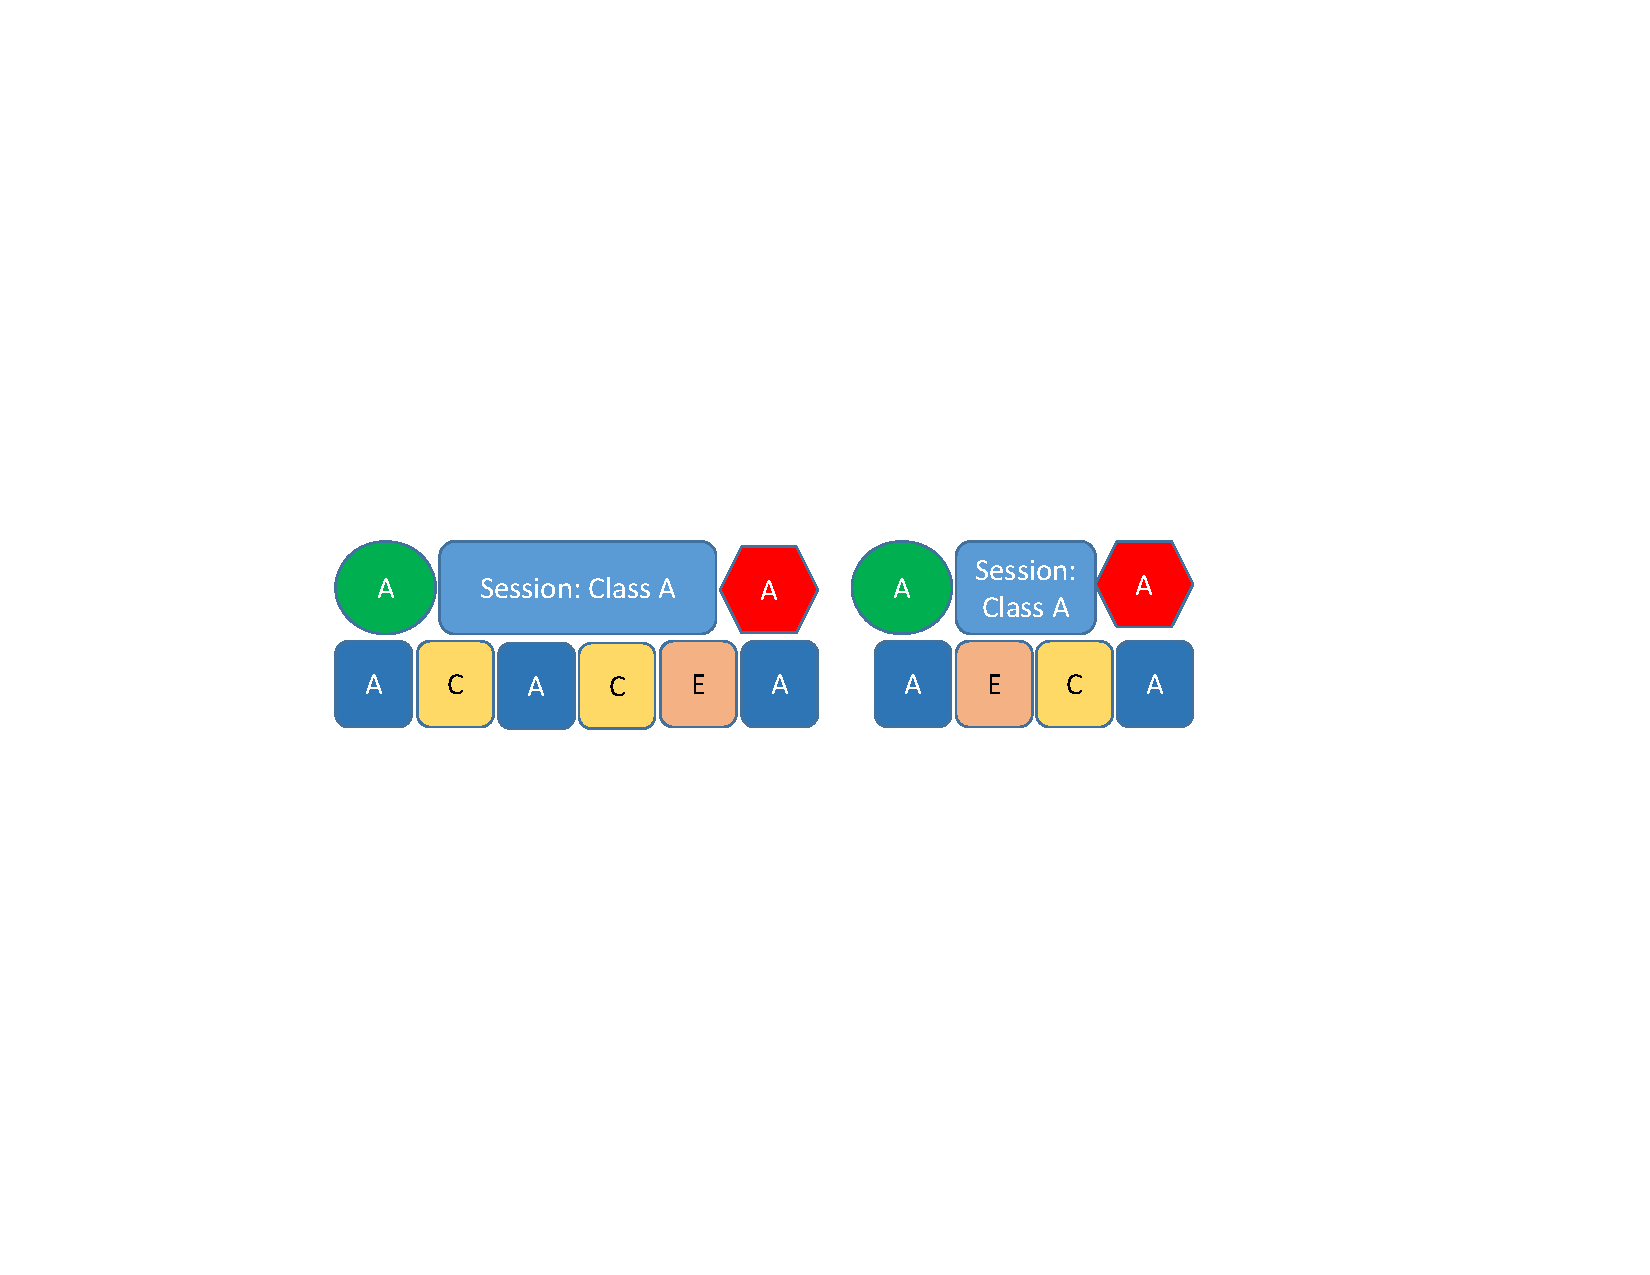
\includegraphics[width=\linewidth]{SessionDataConcept.pdf}
	\caption{Conceptual View of Sessions}
	\label{fig:SessionDataConcept}
\end{figure}

\Fix{The following is unclear in the context of block and super block}
When sessions repeat, additional or fewer classes may be viewed by the developer, regardless they incur some comprehension effort which we add to the interest payments.  In each session, we determine the interest amount from the comprehension data quantifying it in hours. 


Within a session, we calculate measurements related to comprehension effort as follows:
\begin{itemize}
	\item[] $Number of sessions$ is the number of time window sessions formed by each class 
	\item[] $Count Number of Class Visits$ is the number of times the class itself has been accessed inside a session \Fix{Will:changed Edits to Visits..I think we mean visits?}
	\item[] $Count Number of Other Class Accesses$ is the number of unique files visited in each session
	\item[] $Time Spent in Class$ is the time spent in the class that forms the session
	\item[] $Time Spent in Other Classes$ is the time spent in all other files in the session
\end{itemize}

  

The framework matches the comprehension data with code structure data at the class level.  Therefore we consider class level code structure metrics whose definitions align with the measurements taken for comprehension.  Data for code structure is provided by the $Understand$ tool from Scientific Tool Works.  The framework used the following metrics for code structure data at the class level:

\begin{itemize}
	\item[] $Count Class Coupled$ is the number of other classes coupled to
	\item[] $Count Class Base$ is the Number of immediate base classes
	\item[] $Count Class Derived$ is the number of immediate sub-classes
	\item[] $Count Declared Method$ is the number of local methods for the class
\end{itemize}

The class level metrics for code structure are related to comprehension metrics through the name of the source file in the $Blaze$ data corresponding to the class.  In cases where the source file contains multiple classes, the structure metrics were aggregated.

Aligning these two data sources at the module level allows us to ask questions of the intersected data set.  For example, we find the following questions interesting:

\begin{itemize}
	\item[] How much time does the developer spend understanding the code related to the change they are making?
	\item[] How many code elements does the developer need to review related to the change?
	\item[] How many dependent classes does the developer need to review related to the change?
	\item[] How correlated are comprehension effort metrics with code structure metrics?
	\item[] As code structure metic values change, is the corresponding change in comprehension effort linear or non-linear.
\end{itemize}

\section{Analysis}
\label{sec:AnalysisResults}
\begin{center}
\begin{table*}[t]
	\centering
	\caption{Class Data for Each Developer}
	\begin{tabular}{|l|l|l|l|l|l|l|}
	\hline

Developer Name & Class Name & No Of Blocks &Count No of Class Edits & Count No of Other Class Accesses & Time Spent in Class & Time Spent in Other Classes\\
\hline\hline
Developer X & A & 74 & 294 & 78 & 39hours 34mins 23 secs & 16hours 39mins 36secs\\
\hline
Developer X & B & 32 & 88 & 52 & 2hours 54mins 20 secs & 8hours 54mins 18secs\\
\hline
Developer X & C & 28 & 77 & 52 & 4hours 28mins 25 secs & 9hours 15mins 41secs\\
\hline
Developer Y & P & 10 & 45 & 24 & 2hours 19mins 13 secs & 1hour 43mins 12secs\\
\hline
Developer Y & Q & 7 & 12 & 20 & 24 mins 08 secs & 2hours 36mins 32secs\\
\hline
Developer Y & R & 5 & 15 & 16 & 53 mins 51 secs & 40mins 18secs\\
\hline

	\end{tabular}
	\label{fig:AnalysisData}
\end{table*}
\end{center}

As previously mentioned we first define sessions to investigate each class that a developer visits. We define session as a moving window time where developer is investigating a certain class. When we define a session of X hours for a class Y we mean to say that starting from the first time the developer visits class Y while navigating we find the last time he visits the same class in X hours. We refer to this unit as a  "block" for the class that we want to study. For each block of class Y that we obtain we study the number of unique classes the developer has visited while in the block as well as the number of times the developer has visited the class Y iteslf within the block. The classes central to a task will have a high count of the number of times the developer visits the class in a particular block and the number of such blocks will also be high. We also calculate the time spent by developer in the central class as well as the time spent by the developer spent in other classes in the block of the central class.The time factor gives us an estimation of how well the developer comprehends the class and other classes referenced in the block. We studied such blocks for a moving window of 4 hours, 8 hours, 12 hours and 16 hours. 

The data collected by the Blaze logs has all the navigation activities done by the developer in the IDE. It also has appropriate time outs for periods of inactivity in the IDE. We first filtered out all the navigation activities related to classes as well all time outs and IDE exits. Next we calculated the time spent by the developer in the class. We obtained a list of such classes and the time spent by the user in each class. We observed there were instances when the developer accessed a class for less than a second and then switched to another class. We assumed that no useful comprehension can be done by the user in less than a second and attributed such class accesses to random clicks and removed all such entries. We then calculated various parameters that would help in identifying the central class as well the neccesary classes for comprehending the central class. For each sliding window size we calculated the following parameters:
\begin{itemize}
	\item[] Number of blocks formed by each class (No Of Blocks).
	\item[] Number of times the class itself has been accessed inside the block (Count No of Class Edits).
	\item[] Number of unique files visited in each block (Count No of Other Class Accesses).
	\item[] Time spent in the class that forms the block (Time Spent in Class).
	\item[] Time spent in all other files in the block (Time Spent in Other Classes). 
\end{itemize}
We observed that there was a small change in the number of blocks formed by each class between the 4 hour moving window and the 8 hour moving window. The fact that there is not a huge downslide from the 4 hour window to the 8 hour window means that developers do not very often work in 8 hour windows but rather more often do so in 4 hour windows. The 8 hour moving window formed the same number of blocks as that of the 12 hour and 16 hour window. Since the difference was not much between the 4 hour and 8 hour sliding window we decided to use the 4 hour sliding window for further analysis.

Table~\ref{fig:AnalysisData} shows data for each developer that we investigated. We present 3 classes for each of the developers. Each column represents the 5 parameters we defined to be useful in quantifying the \TD. As you can see for developer X we observe a very high count of the number of blocks as well as high counts in number of class edits and number of other class accesses for Class A. This suggests that the developer referenced Class A over a long period of time and very frequently. The developer also frequently referred to other classes while working on Class A. The data shows that the developer spent more than 39 hours working on Class A and more than 16 hours referencing other classes. The 16 hours the developer spent on other files can be interpreted as a cost of comprehending class A. Thus it can be veiwed as  \TD. Similarly when we see Class B we see that developer X spent nearly 3 hours on Class B but spent nearly 9 hours referencing other classes. This indicates that the developer spent 3 times the time actually spent on the central class in other classes. Only taking time as a factor cannot lead to such conclusions and we need to make sure that the class that we consider as the block is central to the task at hand. In this case the developer has 32 such blocks of Class B where he has also referenced Class B 88 times in these blocks. We can safely say that the developer keeps coming back to class B and thus it must be central to the task. Similar patterns can be seen in developer Y where each parameter is indicative of the fact that the considered class is indeed the central class and that the time spent navigating other classes has a significant impact in calculating \TD.


\section{Conclusions and Future Ideas}
In this paper we proposed a framework in which code maintainability data and comprehension effort data are combined to support continuous updates of interest payment estimates, which in turn supports real-time prioritization of debt removal efforts. The primary contribution of our proposed framework is the integration of developer activity data with static code metrics and the concomitant improvements in understanding of developer comprehension effort and in the accuracy with which interest payments can be estimated. An initial investigation of data that we collected from ABB developers demonstrates the feasibility of the framework and provides examples of how the developer activity data work in concert with structural code metrics to reveal new information about developer comprehension effort.

Our next step will be to conduct a large-scale statistical analysis of comprehension and structural metrics to better understand the correlations and levels of technical debt that drive increased comprehension effort.  With this analysis we will determine how to calculate interest payments for technical debt items.  This will include resolving what portion of comprehension effort is for technical debt and the portion that is inherent in comprehending the ideal code structure.  

We plan to further develop the framework and to use it to answer a number of questions about the relationships between developer comprehension effort and technical debt.  For example, we plan to include other comprehension metrics such as the number of edits to a class that will allow evaluation of the Shotgun Surgery smell where multiple classes are modified for a change.  To improve the accuracy of the comprehension data, we plan to detect the central class based on edit actions as well as navigation and search actions during a session.  We also plan to conduct an observational study of developers to validate the estimates  of interest payments during maintenance activities.

\section*{Acknowledgment}
The authors would like to thank ABB Corporate Research for supporting this work.

%\IEEEtriggeratref{8}
\bibliographystyle{IEEEtran}
\bibliography{Monitoring,wbsnipes-td,nkraft}

\end{document}
